\documentclass[ %
    11pt, %
    a4paper, %
    BCOR=12mm, %
    DIV=12, %
    headsepline=true, %
    parskip=half, %
    %draft=true, %
]{article}

\usepackage[utf8]{inputenc}
\usepackage[T1]{fontenc}
\usepackage{lmodern}
%%englisches Protokoll
\usepackage[british,UKenglish,USenglish,english,american]{babel}
% %
%%deutsches Protokoll
%\usepackage[ngerman]{babel}
% %
\usepackage{amssymb,amsmath}
\usepackage{engrec}
\usepackage{enumerate}
\usepackage{empheq}
%\usepackage{picins}
\usepackage{floatflt}
\usepackage{graphicx}
\usepackage{color}
\usepackage{natbib}
\usepackage{pdfpages}
\usepackage{hyperref}
\graphicspath{{Bilder/}}%% Allgemeine Bilder
\usepackage[paper=a4paper,left=25mm,right=25mm,top=25mm,bottom=25mm]{geometry}

\begin{document}


\begin{titlepage}

\begin{center}




\includegraphics[width=0.3\textwidth]{Bilder/logo}\\[1.2cm]    

\textsc{\LARGE Albert-Ludwigs-Universit\"at Freiburg}\\[1.75cm]

\textsc{\Large Physikalisches Fortgeschrittenen-Praktikum I}\\[0.75cm]



\newcommand{\HRule}{\rule{\linewidth}{0.5mm}}
\HRule \\[0.5cm]
{ \huge \bfseries Szintillationszähler}\\[0.5cm]

\HRule \\[1.75cm]


\begin{minipage}{0.4\textwidth}
\begin{flushleft} \large
\emph{Studenten:}\\
Daniel \textsc{Uhl}\\ \setlength{\parindent}{1.25cm} \& 
\setlength{\parindent}{0cm} \\ Jan P\'eter \textsc{Szabados} 
\end{flushleft}
\end{minipage}
\hfill
\begin{minipage}{0.4\textwidth}
\begin{flushright} \large
\emph{Tutor:} \\
Matthias \textsc{Gorzellik}\\
\end{flushright}
\end{minipage}

\vfill


{\large \today}

\end{center}

\end{titlepage}

\pagenumbering{Roman}

\tableofcontents
\newpage
\pagenumbering{arabic}

\section{Theoretische Grundlagen}
\subsection{Supraleiter}
Man nennt Materialien, deren elektrischer Widerstand unterhalb einer materialabhängigen kritischen Temperatur $T_{C}$ unmessbar klein wird, Supraleiter. Dabei verhalten sie sich wie ideale Diamagneten: Wird ein äußeres Magnetfeld angelegt, wird ein Strom in dem Supraleiter induziert, sodass im Inneren des Leiters ein Magnetfeld induziert wird, welches das äußere Feld genau kompensiert. Bei der Verdrängung Magnetfeldes aus dem Inneren des Supraleiters spricht man vom 'Meissner-Ochsenfeld-Effekt'.\\
Das Prinzip der Supraleitung basiert auf sogenannten 'Cooper-Paaren', makroskopischen Zuständen von zwei Elektronen, welche über hunderte Nanometer hinweg miteinander verbunden sind. Die Entstehung und Wirkung der Cooper-Paare wird durch die sogenannte 'BCS-Theorie' beschrieben, welche noch ausführlich diskutiert wird.\\
Es kann durch steigende Temperatur (für $T>T_{C}$), aber auch durch große externe Ströme, ein starkes äußeres Magnetfeld oder ein externes elektromagnetisches Wechselfeld der Größenordnung $\omega\approx \Delta E/\hbar$, mit welchem Elektronen über die 'Bandlücke' des Supraleiters angeregt werden, die Supraleitung unterbrochen werden.\\
~\\
Es werden zwei Arten von Supraleitern unterschieden:\\
\textbf{Typ I}\\
Das innere Magnetfeld sinkt unterhalb einer kritischen äußeren Magnetfeldstärke $H_{C}$ auf 0 (wenn $T<T_{C}$). Das Magnetfeld dringt  nur wenige Nanometer in den Leiter ein.\\
~\\
\textbf{Typ II}\\
Diese Art von Supraleiter wird auch 'Hochtemperatursupraleiter' genannt, da die kritischen Temperaturen deutlich höher sind als diejenigen für Supraleiter von Typ I. \\
Es werden zwei Stufen für das innere Magnetfeld unterschieden:  Unterhalb der externen Feldstärke $H_{C_{2}}$ sinkt die innere Feldstärke auf kleine Werte, unterhalb von $H_{C_{1}}$ auf null. Zwischen diesen beiden Feldstärken kommt es zur Bildung von Flussfäden im Leiter, welche lokal für einen kleinen Feldbeitrag sorgen. 
\subsection{BCS-Theorie}
Wie bereits erwähnt, wird die Supraleitung mittels Cooper-Paare, welche aus zwei Elektronen bestehen, die über hunderte Nanometer miteinander wechselwirken, durch die BCS-Theorie (benannt nach ihren Entwicklern John \textbf{B}ardeen, Leon N. \textbf{C}ooper und John R. \textbf{S}chrieffer) erklärt.\\
Die gegenseitige Anziehung der Elektronen beruht auf der Trägheit der positiv geladenen Atomrümpfe. Kommt es zu Gitterschwingungen im Kristall, so wandern die Atomrümpfe langsamer in ihre Ausgangsposition zurück als die Elektronen. Aus diesem Grund ziehen - bildlich gesprochen - Elektronen einen Schweif positiver Polarität hinter sich her. Dieser kann ein Elektron ähnlicher Energie und entgegengesetztem Spin anziehen, wodurch sich ein Cooper-Paar bildet. \\
Um möglichst viele solche Paare zu erhalten, muss eine tiefe Temperatur vorherrschen, damit alle Zustände bis zur Fermi-Energie gefüllt sind. Auf diese Weise gibt es viele Elektronen ähnlicher Energie und kaum thermische Anregung: Die schwache Wechselwirkung zwischen den beiden Elektronen, welche das Cooper-Paar formen, wird also nicht aufgebrochen. Die einzelnen Elektronen bilden nun nicht mehr Fermionen, sondern dank der Spinkopplung miteinander ein Boson. Die Wechselwirkungsenergie ist dabei kleiner als die der einzelnen Ladungsträger.\\
Da die Bosonen nicht dem Pauli-Prinzip unterliegen, können beliebig viele Cooper-Paare denselben Zustand, auch den Grundzustand, einnehmen. Dadurch kommt es zu keiner Wechselwirkung mit dem Rest des Leiters mehr, was der Grund für den unmessbar kleinen elektrischen Widerstand ist. \\
Kommt es zum Zusammenbrechen der Supraleitung, werden eigentlich die Cooper-Paare aufgebrochen. Bei dem Entstehen eines Cooper-Paares wird Energie frei. Wird diese Energie einem Cooper-Paar zugeführt, kann dieses aufgebrochen werden. Unterschiedliche Methoden hierfür wurden im Unterkapitel 'Supraleiter' beschrieben.
\subsection{Flussquantisierung}
Der in diesem Versuch verwendete Supraleiter hat die Form eines Ringes. Der magnetische Fluss kann somit mithilfe des Stoke'schen Satzes über das geschlossene Integral des Vektorfelds $\vec{A}$ über die Leiterschleife berechnet werden: 
\[\oint\vec{A}d\vec{l}=\Phi_{B}.\]
Da sich, wie bereits diskutiert, alle Cooper-Paare im gleichen Zustand befinden, können sie als Gesamtwelle betrachtet werden. Somit ist es klar, dass sich die Phase $\theta$ bei einem Umlauf nur um Vielfache von $2\pi$ ändern kann: 
\[\oint\triangledown\theta d\vec{l}=\Delta\theta=n\cdot 2\pi,\] 
wobei $n\in\mathbb{N}$.\\
Somit ergibt sich die Quantisierung des magnetischen Flusses im geschlossenen Supraleiter in sogenannten Flussquanten: 
\[\left|\Phi_{B}\right|=n\frac{\hbar}{2e}=n\Phi_{0},\]
wobei $\Phi_{0}=2,067833667\cdot10^{-15}Tm^{2}$ (Quelle: [ver]).
\subsection{Josephson-Effekt}
Der Josephson-Effekt tritt auf, wenn ein dünner Isolator ('Josephson-Kontakt') zwischen zwei Supraleiter gebracht wird.
\begin{figure}[h]
\begin{center}
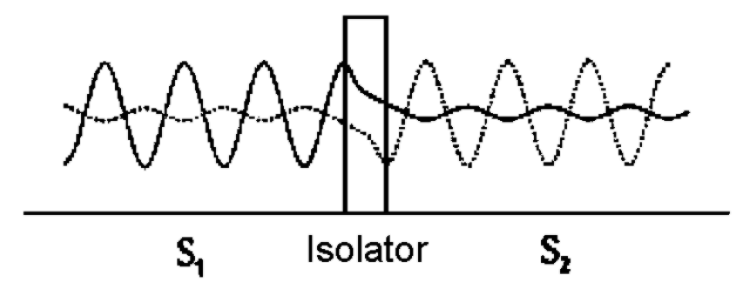
\includegraphics[scale=0.6]{Bilder/josephson}
\caption{Josephson-Kontakt zwischen zwei Supraleitern. Quelle: [ver].}
\end{center}
\end{figure}
~\\
Aufgrund der geringen Breite des Kontakts (wenige Nanometer) können Cooper-Paare mit hoher Wahrscheinlichkeit durch ihn tunneln, wodurch ein Tunnelstrom verursacht wird.\\
Wenn der Josephson-Kontakt, wie in diesem Experiment, zwischen zwei identischen Supraleitern ohne Potentialdifferenz liegt (dies ist hier der Fall wegen der Ringform des Supraleiters), so hängt der Tunnelstrom ausschließlich von der Phasendifferenz der einlaufenden Wellen ab. Der Josephson-Kontakt verhält sich zwar für den Strom wie ein schwacher Supraleiter, kann aber dennoch von einem äußeren Magnetfeld durchdrungen werden. Dadurch kann die Kopplung der Wellen und ihre Phasenlage verändert werden. \\
Solange sich das Material im supraleitenden Zustand befindet, fließt ein Gleichstrom von tunnelnden Cooper-Paaren, der 'Josephson-Gleichstrom' genannt wird. Wird aber eine kritische Stromstärke $I_{C}$ überschritten, so beginnen die Cooper-Paare aufzubrechen. \\
Der Tunnelstrom/'Josephson-Gleichstrom' kann in Abhängigkeit eines äußeren magnetischen Flusses $\Phi_{m}$ und dem Flussquant folgendermaßen geschrieben werden:
\[I=I_{0}\cdot\frac{sin(\pi\Phi/\Phi_{0})}{\pi\Phi/\Phi_{0}}.\] 
Der dazugehörige Graph sieht folgendermaßen aus:
\begin{figure}[h]
\begin{center}
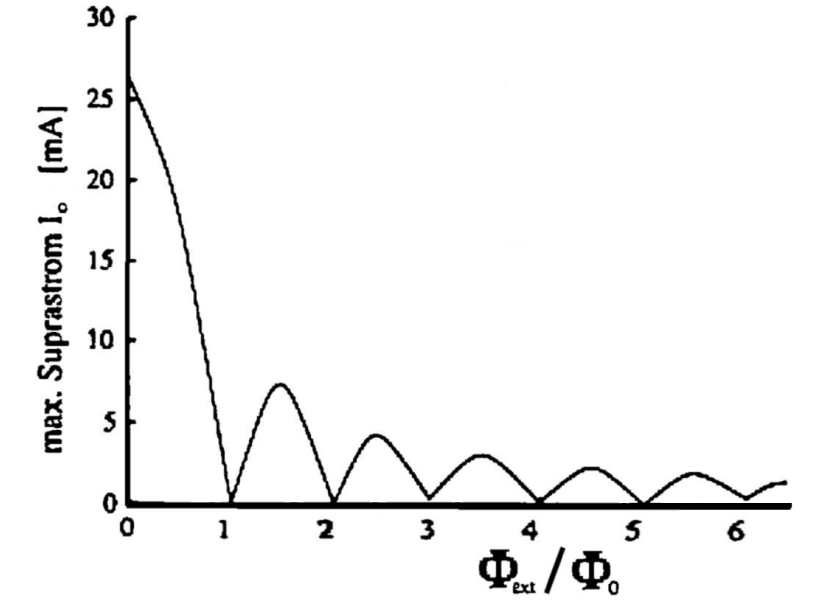
\includegraphics[scale=0.6]{Bilder/tstrom}
\caption{Maximaler Tunnelstrom durch den Josephson-Kontakt in Abhängigkeit des externen magnetischen Flusses. Quelle: [ver]}
\end{center}
\end{figure}
\section{Realization}
\subsection{Experimental Setups}
%Bilder
The permanent magnetic field is provided by a large electromagnet connected to a power supply. The modulation of the magnetic field is created by two coils on the left and the right side of the sample holder. Those are connected to a sine voltage firstly and an adder at the end. There's an electromagnetic oscillating circuit between the respective ends of the iron cores of the electromagnet. There is a hole in the middle of it where the Hall sensor or the samples can be introduced. It's also connected to a frequency generator. An oscilloscope is connected to the modulating voltage to show its course just as to the oscillating circuit to show resonances.
\subsection{Experimental Approach}
Firstly, the homogeneity of the magnetic field inside the sample holder had to be proven using a Hall sensor. With this measurement, a working point was determined. The setup was the following:\\
\begin{figure}[htbp]
\begin{center}
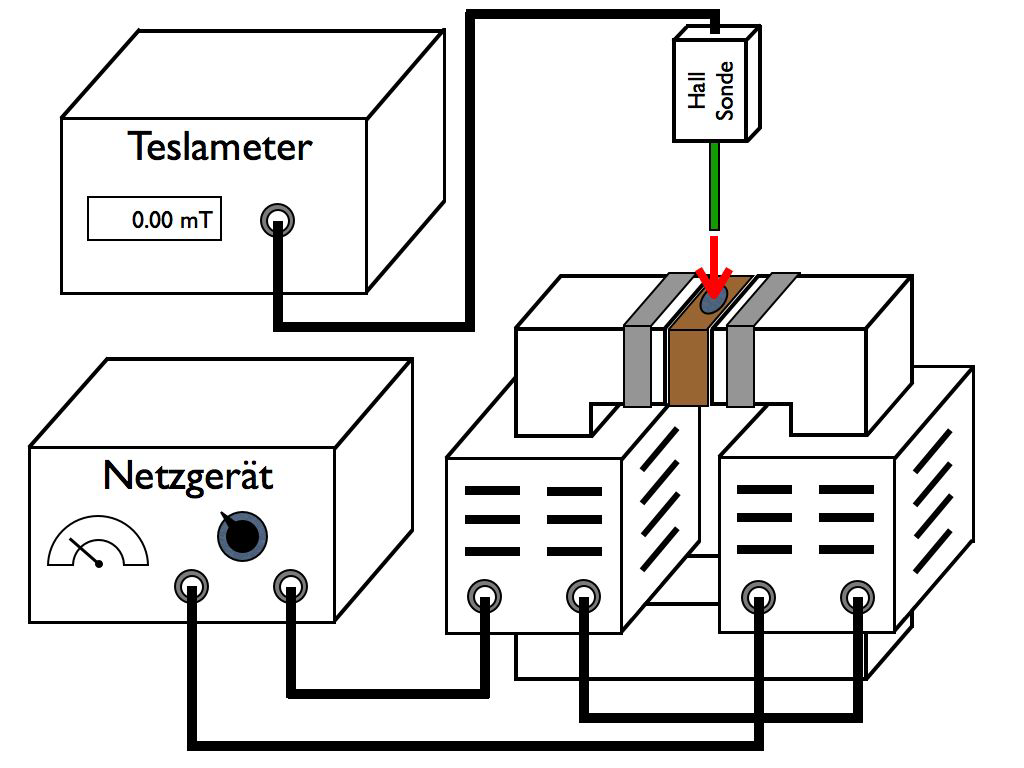
\includegraphics [scale=0.5]{Bilder/hallsonde.png}
\caption{Experimental setup for the determination of the homogeneity of the magnetic field (source: [ver])}
\end{center}
\end{figure}
\clearpage
Afterwards, hydrogen, glycol and Teflon samples were put inside the field one after the other with the intention to find their resonance frequency. A sine modulation was used to facilitate the realization of this part of the experiment: The resonance is passed by twice per sine period. Thus in the resulting absorption curve, one gets two absorption minima. To find the resonance frequency, the minima need to be equidistant, because that way they are at the zero of the modulation, which is at the appointed frequency of the radiation field. The setup and the expected curves can be seen below:\\
\begin{figure}[htbp]
\begin{center}
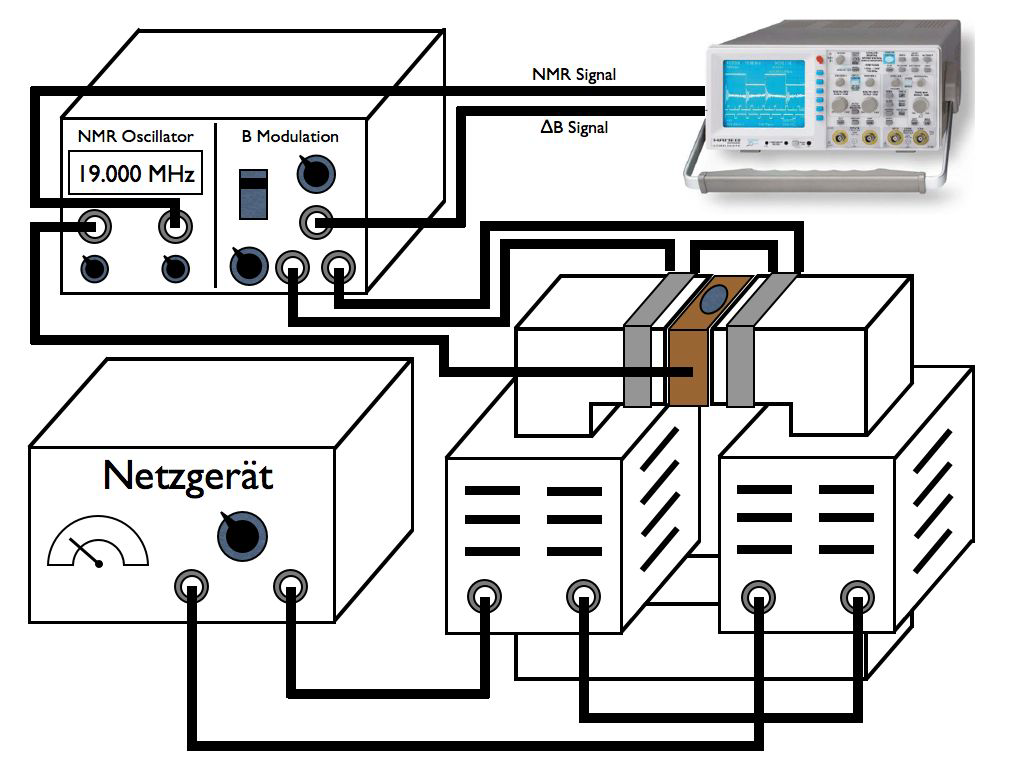
\includegraphics [scale=0.5]{Bilder/teil234.png}
\caption{Experimental setup for the determination of the resonance frequency with the sine-modulation (source: [ver])}
\end{center}
\end{figure}
\begin{figure}[htbp]
\begin{center}
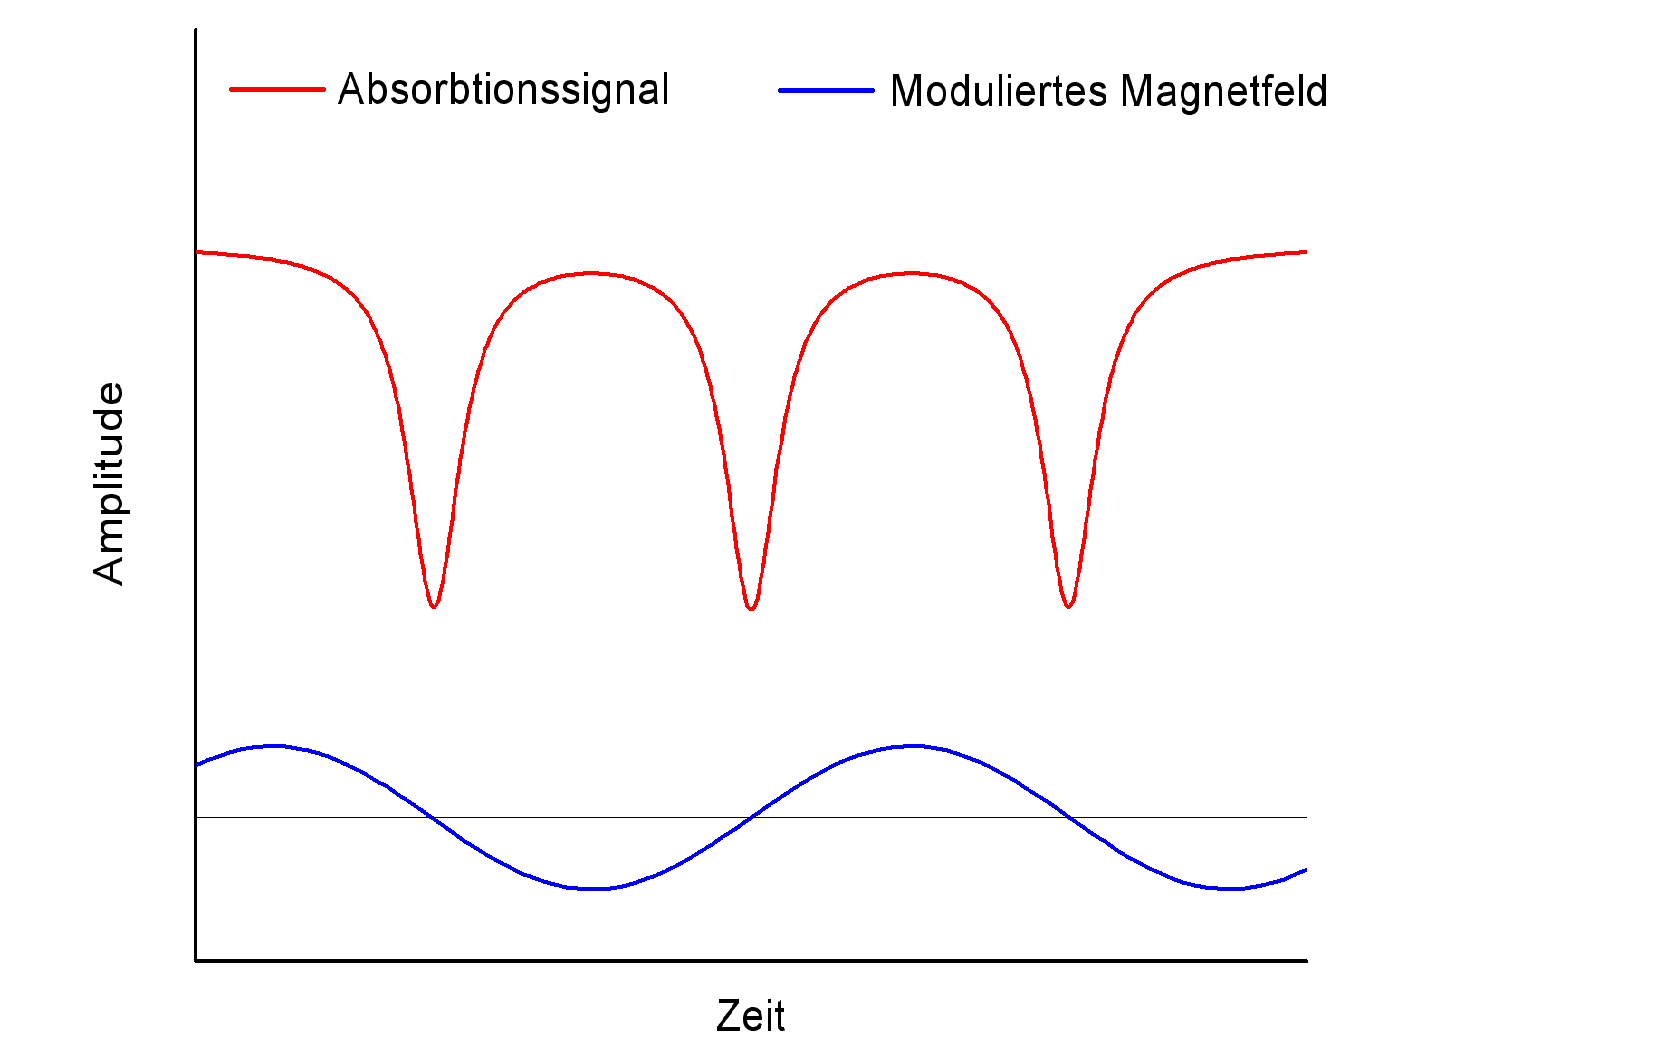
\includegraphics [scale=0.5]{Bilder/theoverlauf1.png}
\caption{Expected curves (source: [ver])}
\end{center}
\end{figure}
\clearpage
To get a better result for hydrogen, we use the lock-in method: a sawtooth voltage is applied as modulation, overlapped by a sine voltage with much lower amplitude and much higher frequency. The differences between the zero of the derived absorption curve and the sine-modulated sawrooth signal in time $\Delta t$ were measured for different frequencies. By using a linear fit, the resonance frequency could be determined (that's the frequency at $\Delta t=0s$). The setup and the expected curves look the following:\\
\begin{figure}[htbp]
\begin{center}
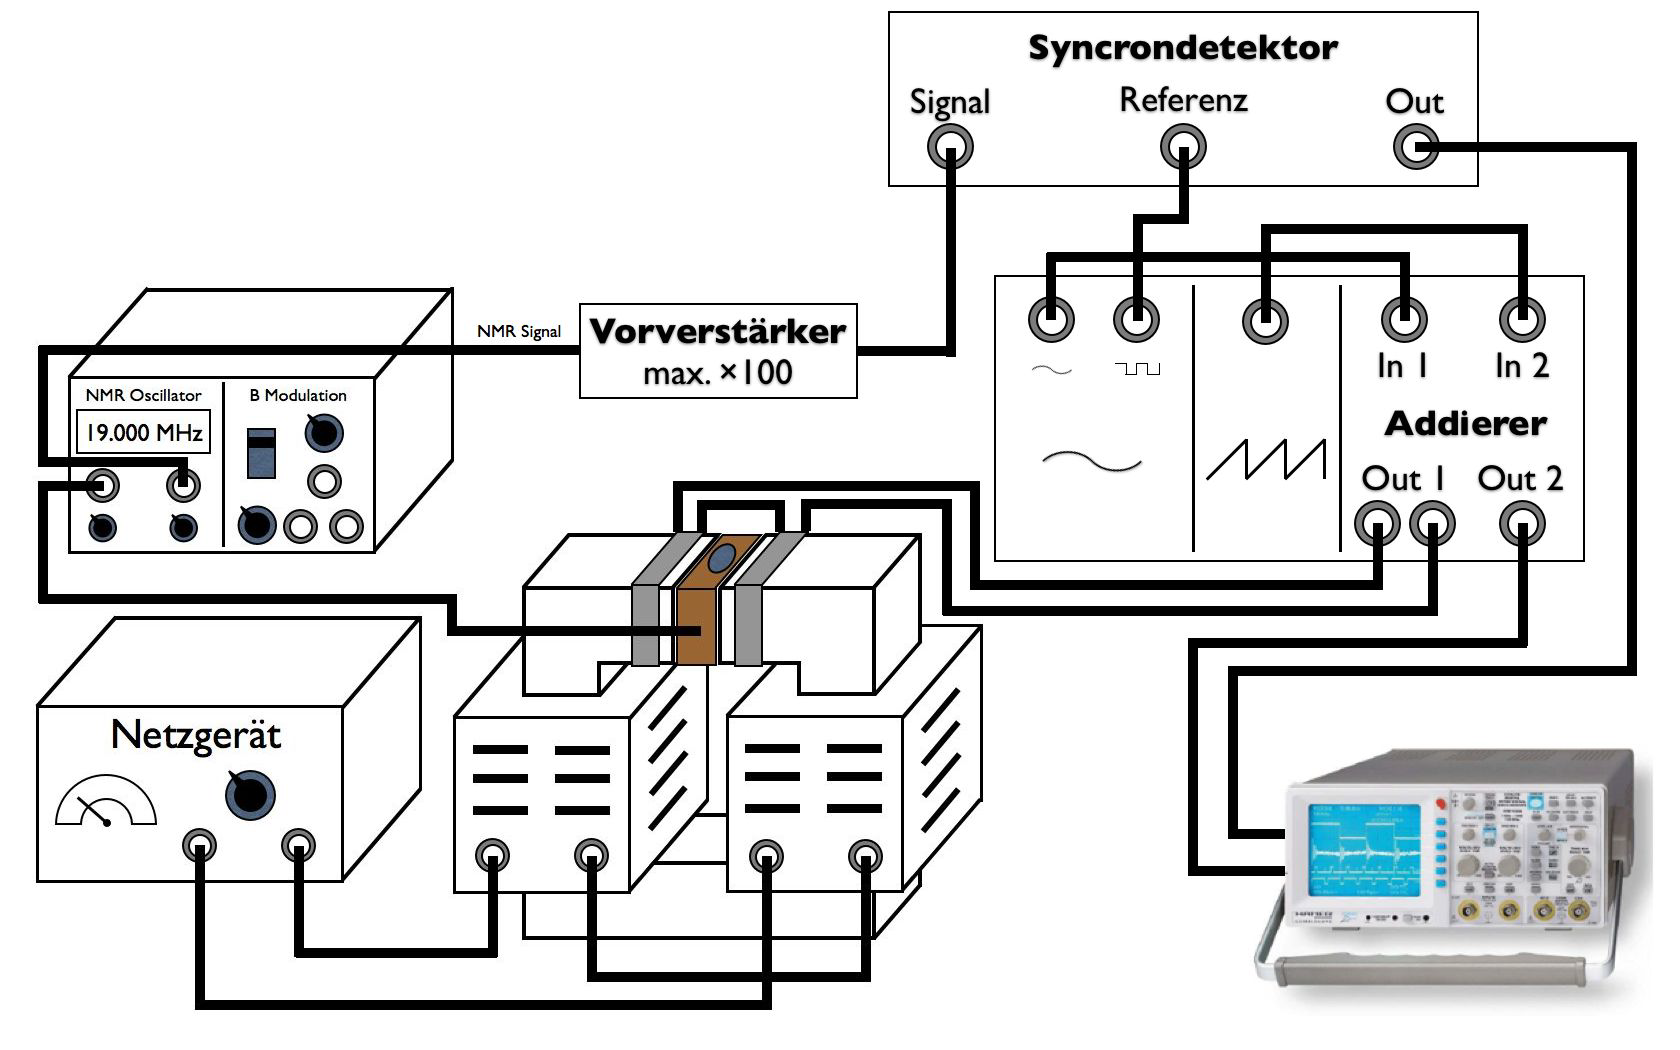
\includegraphics [scale=0.4]{Bilder/lockin.png}
\caption{Lock-in method (source: [ver])}
\end{center}
\end{figure}
\begin{figure}[htbp]
\begin{center}
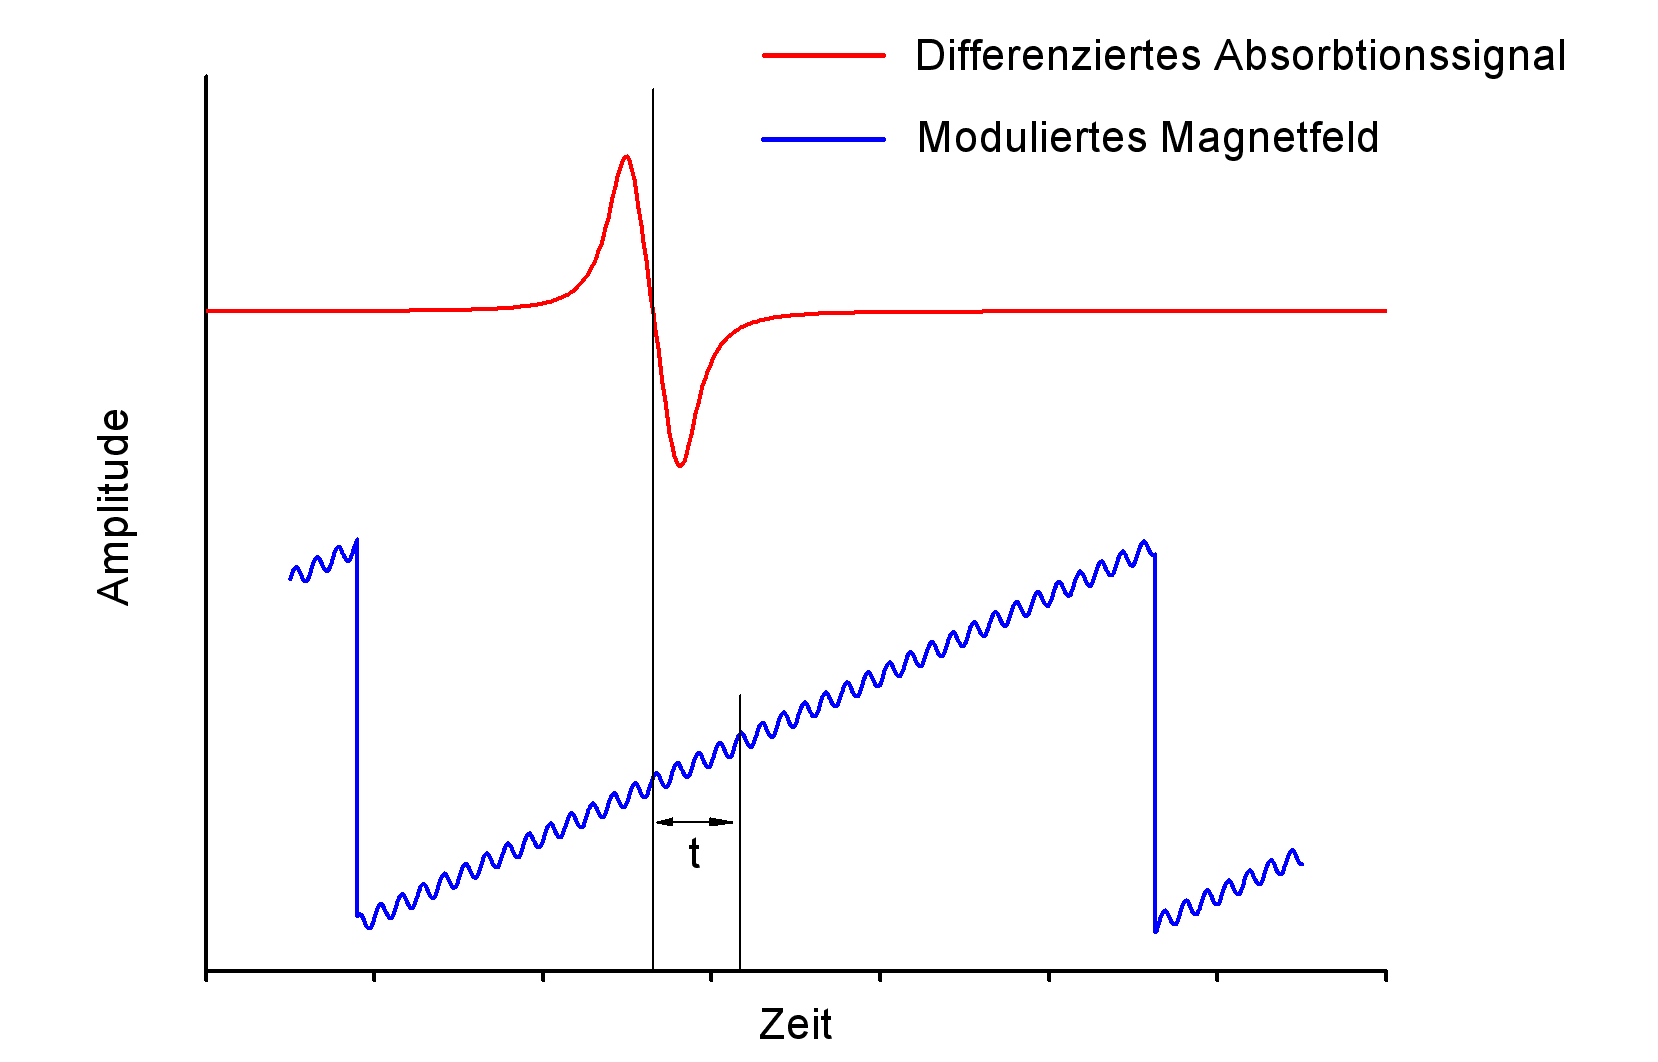
\includegraphics [scale=0.4]{Bilder/theoverlauf2.png}
\caption{Expected curves for the lock-in method (source: [ver])}
\end{center}
\end{figure}
\clearpage

\section{Analysis}
First we will characterize some events by their signature. Unfortunately, this is not sufficient to classify all events
properly from each other, so in the next part we will conduct a serious analysis of the spatial distribution with respect to
the variables measured by the detector. 
\subsection{Signatures of detected particles: Descriptive treatment}
On the next pages figures~\ref{fig:ee},~\ref{fig:mm},~\ref{fig:tt} and~\ref{fig:qq} show
a typical event each of the respective particle. We will not use these figures any
further, but they will give an impression how typical events look like.
The red curves indicate the data of the tracking detector, visualizing the trajectories
in the inner area. Pink squares indicate where the electron calorimeter measured energies
(which we will denote as $E_{\mathrm{ecal}}$)
with the blue squares showing their momentum. Green squares indicate the energy of the
hadron calorimeter (which we will denote as $E_{\mathrm{hcal}}$).

\begin{figure}[htpb]
    \centering
    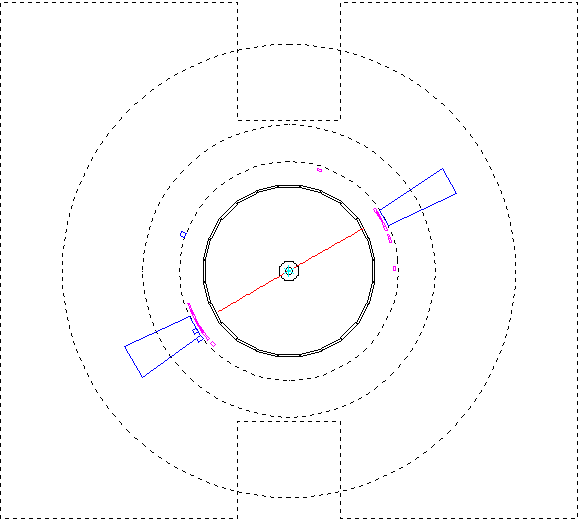
\includegraphics[width=0.8\linewidth]{figures/ee_02.png}
    \caption{Example for typical event of a decay into electrons. The characteristic feature of the decay into electrons is
    the very little number of trajectories and most of the energy submitted to first calorimeter (in the inner circle).}
\label{fig:ee}
\end{figure}

\begin{figure}[htpb]
    \centering
    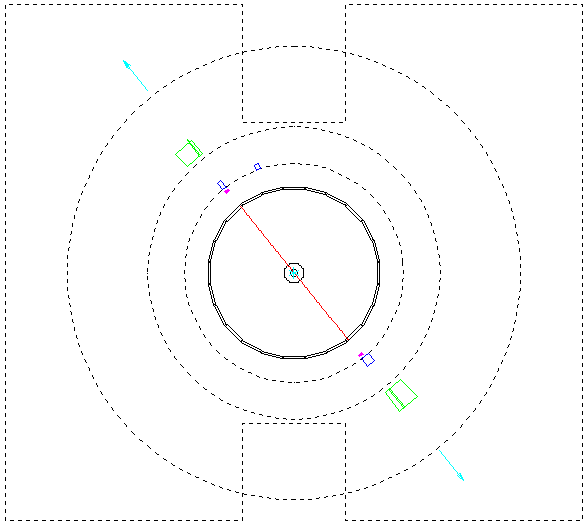
\includegraphics[width=0.8\linewidth]{figures/mm_02.png}
    \caption{Example for typical event of a decay into muons. As muons cannot be bound by the detector most of the time,
        a little amount of energy is absorbed by the first calorimeter. The muon detector far outside of this pictures (which
    is indicated by the turquoise arrows). }
\label{fig:mm}
\end{figure}

\begin{figure}[htpb]
    \centering
    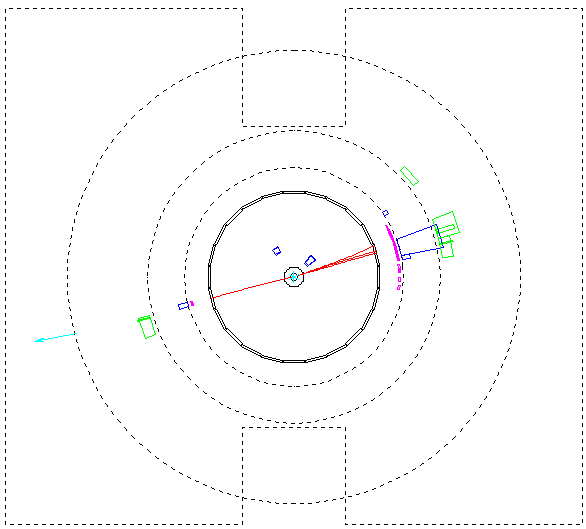
\includegraphics[width=0.8\linewidth]{figures/tt_02.png}
    \caption{Example for typical event of a decay into tauons. As the particles are not
        stopped in the first calorimeter, the probability of being electrons decreases
        significantly (this is not totally true as we will see later). Furthermore,
        there is one particle escaping to the muon detector, but not two in opposite
        directions, as we would expect for muons. There are also no hadron showers
        as characteristic for the quark branch. Hence we conclude this to be a taon event. }
\label{fig:tt}
\end{figure}

\begin{figure}[htpb]
    \centering
    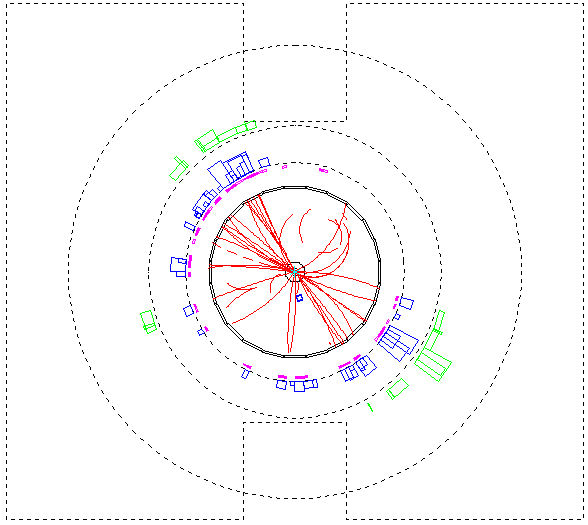
\includegraphics[width=0.8\linewidth]{figures/qq_02.png}
    \caption{Example for typical event of a decay into hadrons. As indicated in figure~\ref{fig:tt} hadronic shower are 
   a signature for quarks, originating from the \textbf{strong confinement}. 
   As bound states of quarks can only be found at low enough
   momentum, we observe a large creation of hadronic particles being
   measured in both of the calorimeter. More than half of
   the energy carried by incident hadrons is passed to additional secondaries. }
\label{fig:qq}
\end{figure}
%TODO
1. More particles, such as photon
2. Experimental setup precise 
we will do that later.


\clearpage
\newpage
\subsection{Monte Carlo data}

\begin{figure}[htpb]
    \centering
    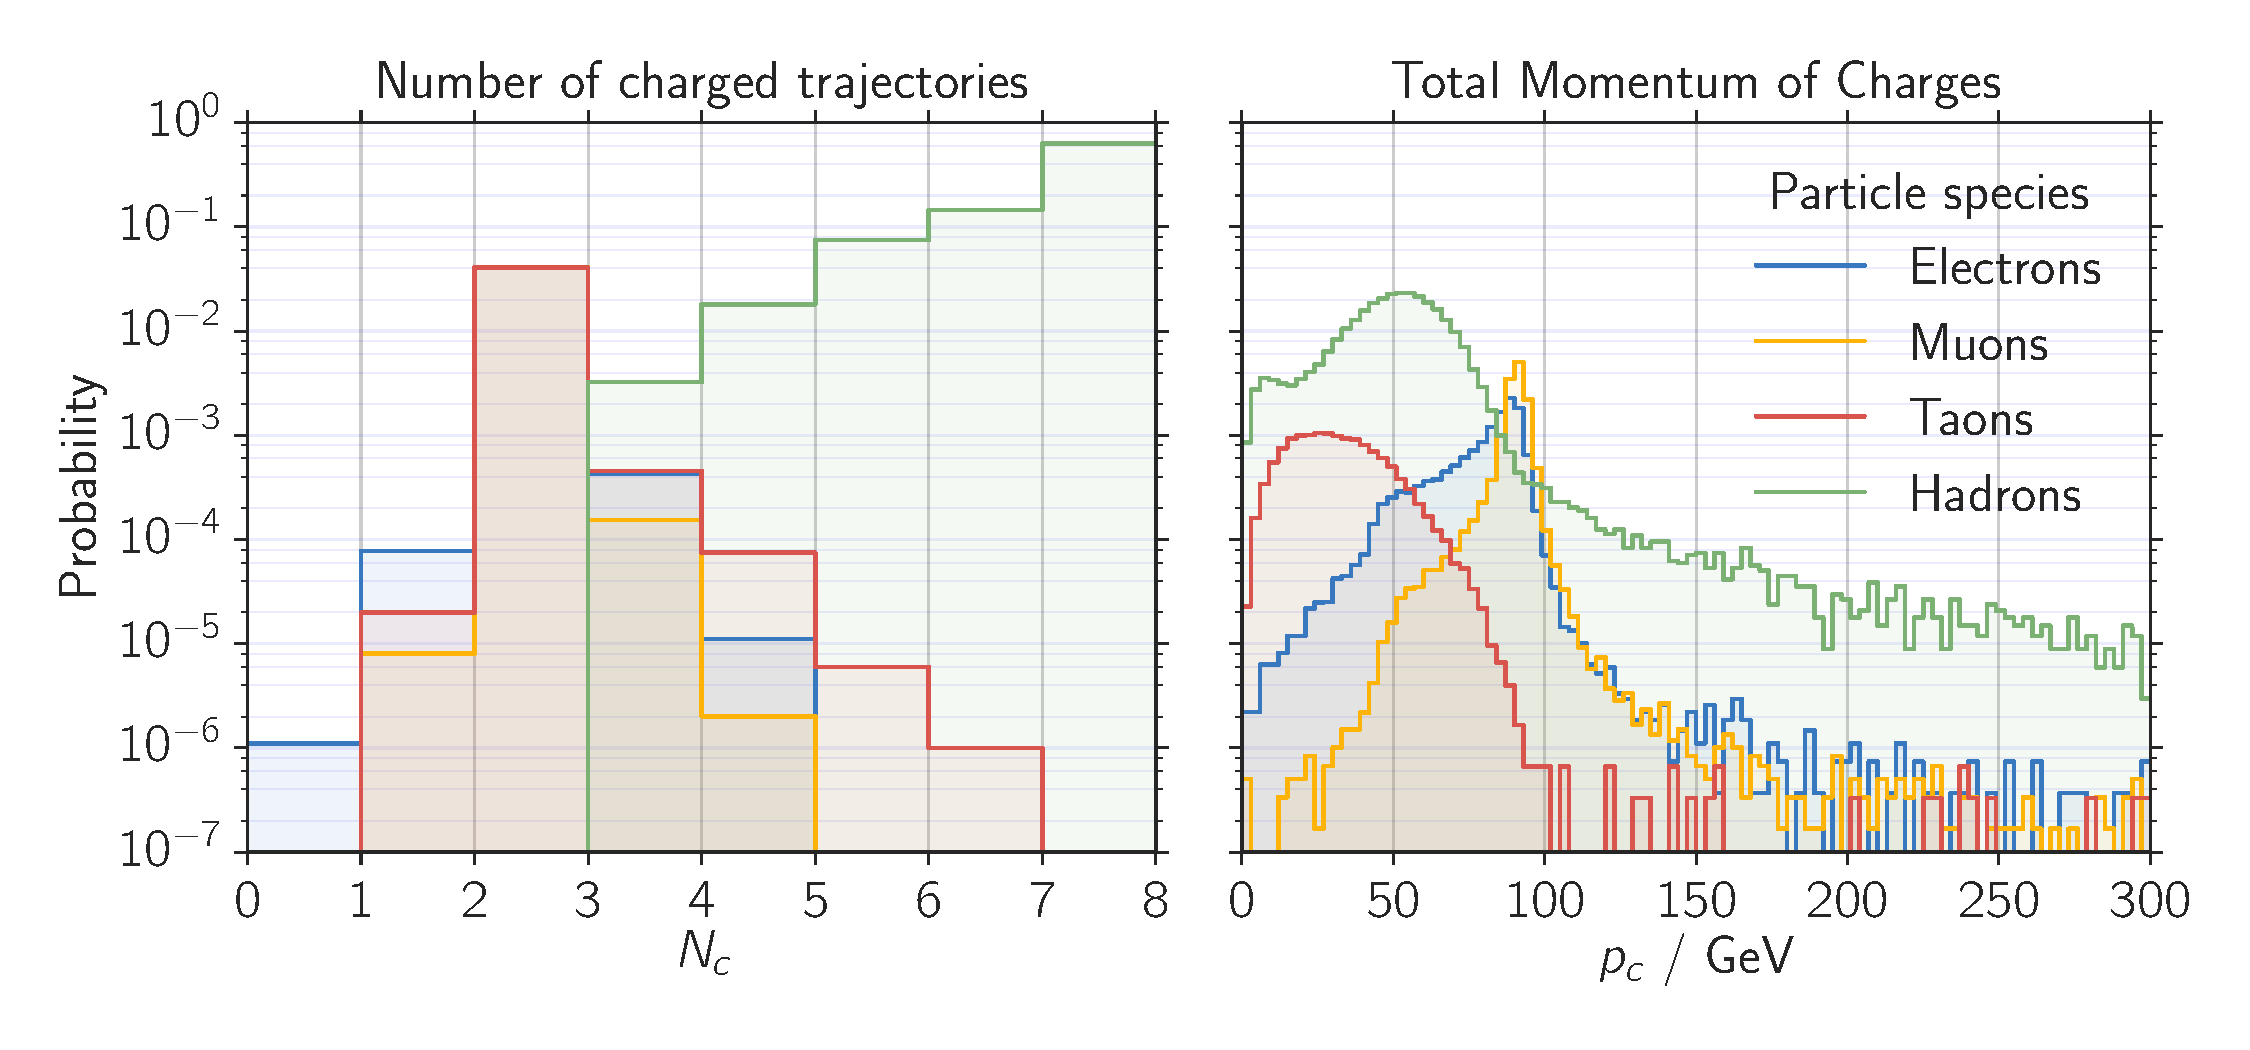
\includegraphics[width=1.0\linewidth]{figures/N_p_c}
    \caption{ bla}
    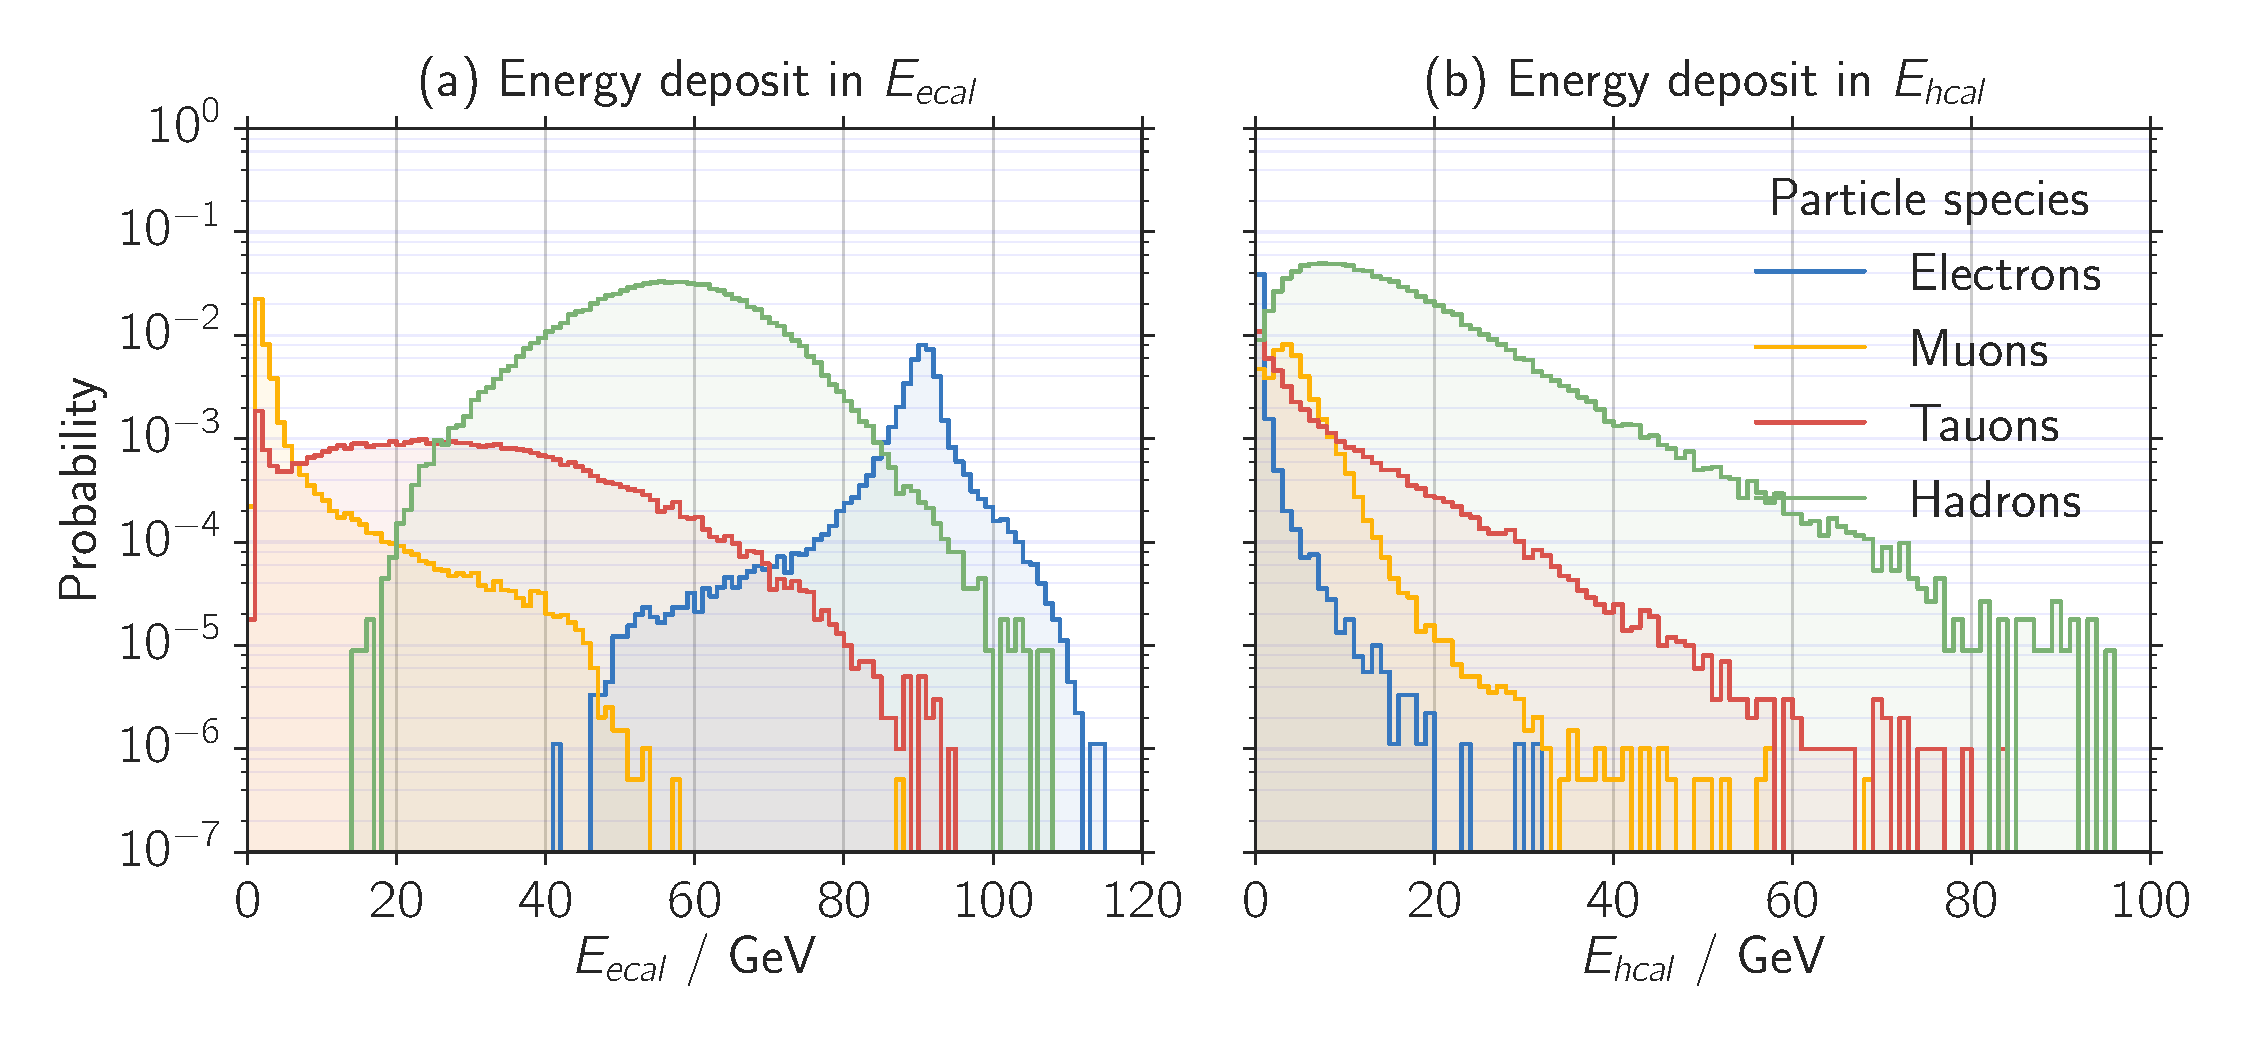
\includegraphics[width=1.0\linewidth]{figures/E_cal}
    \caption{bla}
\label{fig:monte1}
\end{figure}



\subsection{Determination of the Proton Resonance Frequency Using the Lock-in Method}
As already discussed in the "Theoretical Background" chapter, to determine the resonance frequency of a proton in hydrogen using the lock-in method, the zero passages of the sine-overlapped sawtooth voltage and the derived absorption curve had to be measured. The time difference of these had to be determined for different frequencies in order to be able to do a linear fit, with which it was possible to determine the resonance frequency (that's the frequency at $\Delta t=0s$). The frequencies for which we did a measurement can be found in the appendix: as one can see, we decided to neglect the second and third measurement as the chosen frequencies were above the resonance frequency determined in part 2 of the experiment. \\
We determined the zero passage of the derived absorption curve by looking at the two values around the passage. We took the time attached to the closer one and an uncertainty of $s_{t_{abs}}=0,002 s$ as there is a measurement every 0,002 seconds and there might be a deviation for the voltage measured, making it hard to determine the point neighboring the zero passage which is actually closer to 0: this is why we decided to take this uncertainty, the time between two measurements. As for the sine-overlapped sawtooth voltage it was quite hard to determine a zero passage, we decided to determine the period of the signal and add half of it onto the lower end (the start)  of the signal. \\
The period was determined as can be seen below:\\
\[T=t_{top}-t_{bottom}\] where $t_{top}$ stands for the time attached to the maximum voltage and $t_{bottom}$ for the time attached to the minimum voltage reached by the sine-modulated sawtooth signal. Again, we decided to use an uncertainty of $s_{t_ {top}}=s_{t_{bottom}}=0,002 s$ because we don't know about what is happening between the minimum and the maximum of the signal and therefore can't decide, where the actual starting and ending points are. Therefore, the resulting uncertainty can be calculated the following way:\\
\[s_{T}=\sqrt{s_{t_{top}}^{2}+s_{t_{bottom}}^{2}}\]
The period was determined 6 times: we would get $T=5,251 s$ in every measurement. The resulting uncertainty reduces to \[s_{\bar{T}}=\frac{\sqrt{s_{t_{top}}^{2}+s_{t_{bottom}}^{2}}}{\sqrt{6}},\] whereas the period is \[\bar{T}=\frac{1}{6}\sum\limits_{i=1}^{6}T_{i}=5,251 s.\]
As the uncertainty on $t_{bottom}$, $s_{t_{bottom}}=0,2 s$ is not independent of the uncertainty on $\bar{T}$ and that uncertainty is smaller, we decided to neglect $s_{\bar{T}}$, when determining the uncertainty on \[t_{0_{sawtooth}}=t_{bottom}+\bar{T},\] making the resulting uncertainty look like the following:\[s_{t_{0_{sawtooth}}}\approx s_{t_{bottom}}\]
\clearpage
A measurement can be seen below:\\
\begin{figure}[htbp]
\begin{center}
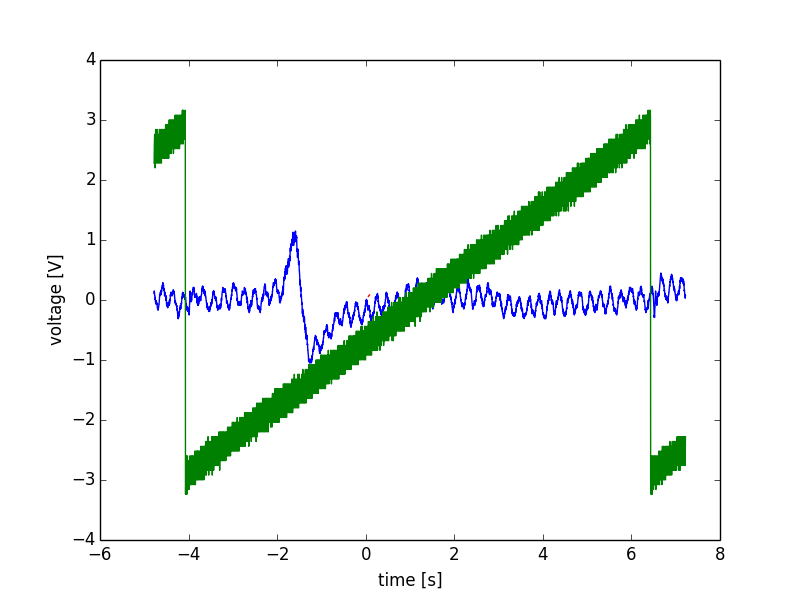
\includegraphics{saege}
\caption{Sine-overlapped sawtooth signal (green) and resulting derived absorption curve (blue)}
\end{center}
\end{figure}
\clearpage
This fits the theoretical expectation, which can be found in the "Theoretical Background" chapter, well.\\
To determine $\Delta t$, we have to calculate the difference between the zero passages of the sine-overlapped sawtooth and the derived absorption signal: \[\Delta t=t_{0_{sawtooth}}-t_{0_{abs}}\] with\\
 \[s_{\delta t}=\sqrt{s_{t_{0_{sawtooth}}}^{2}+s_{t_{0_{abs}}}^{2}}\]
 With the formula and the method explained above we got the following results:\\
 \begin{table}[htbp]
 \begin{center}
 \begin{tabular}{|r|r|r|r|}
 \hline
 \multicolumn{1}{|l|}{f in MHz} & \multicolumn{1}{l|}{$s_{f}$ in MHz} & \multicolumn{1}{l|}{$\Delta t$ in s} & \multicolumn{1}{l|}{$s_{\Delta t}$ in s} \\ \hline
 17,624 & 0,01 & 0,271 & 0,00283 \\ \hline
 17,618 & 0,01 & 0,285 & 0,00283 \\ \hline
 17,6042 & 0,01 & 2,219 & 0,00283 \\ \hline
 17,5998 & 0,01 & 4,195 & 0,00283 \\ \hline
 17,5797 & 0,01 & 4,315 & 0,00283 \\ \hline
 17,6019 & 0,01 & 3,475 & 0,00283 \\ \hline
 17,5892 & 0,01 & 4,017 & 0,00283 \\ \hline
 \end{tabular}
 \end{center}
 \end{table}
 
 We used the displayed values to do our linear fit. The uncertainty we attach to the frequency has already been discussed. Using this values, we did the linear fit mentioned. It can be seen below:\\
 \begin{figure}[htbp]
 \begin{center}
 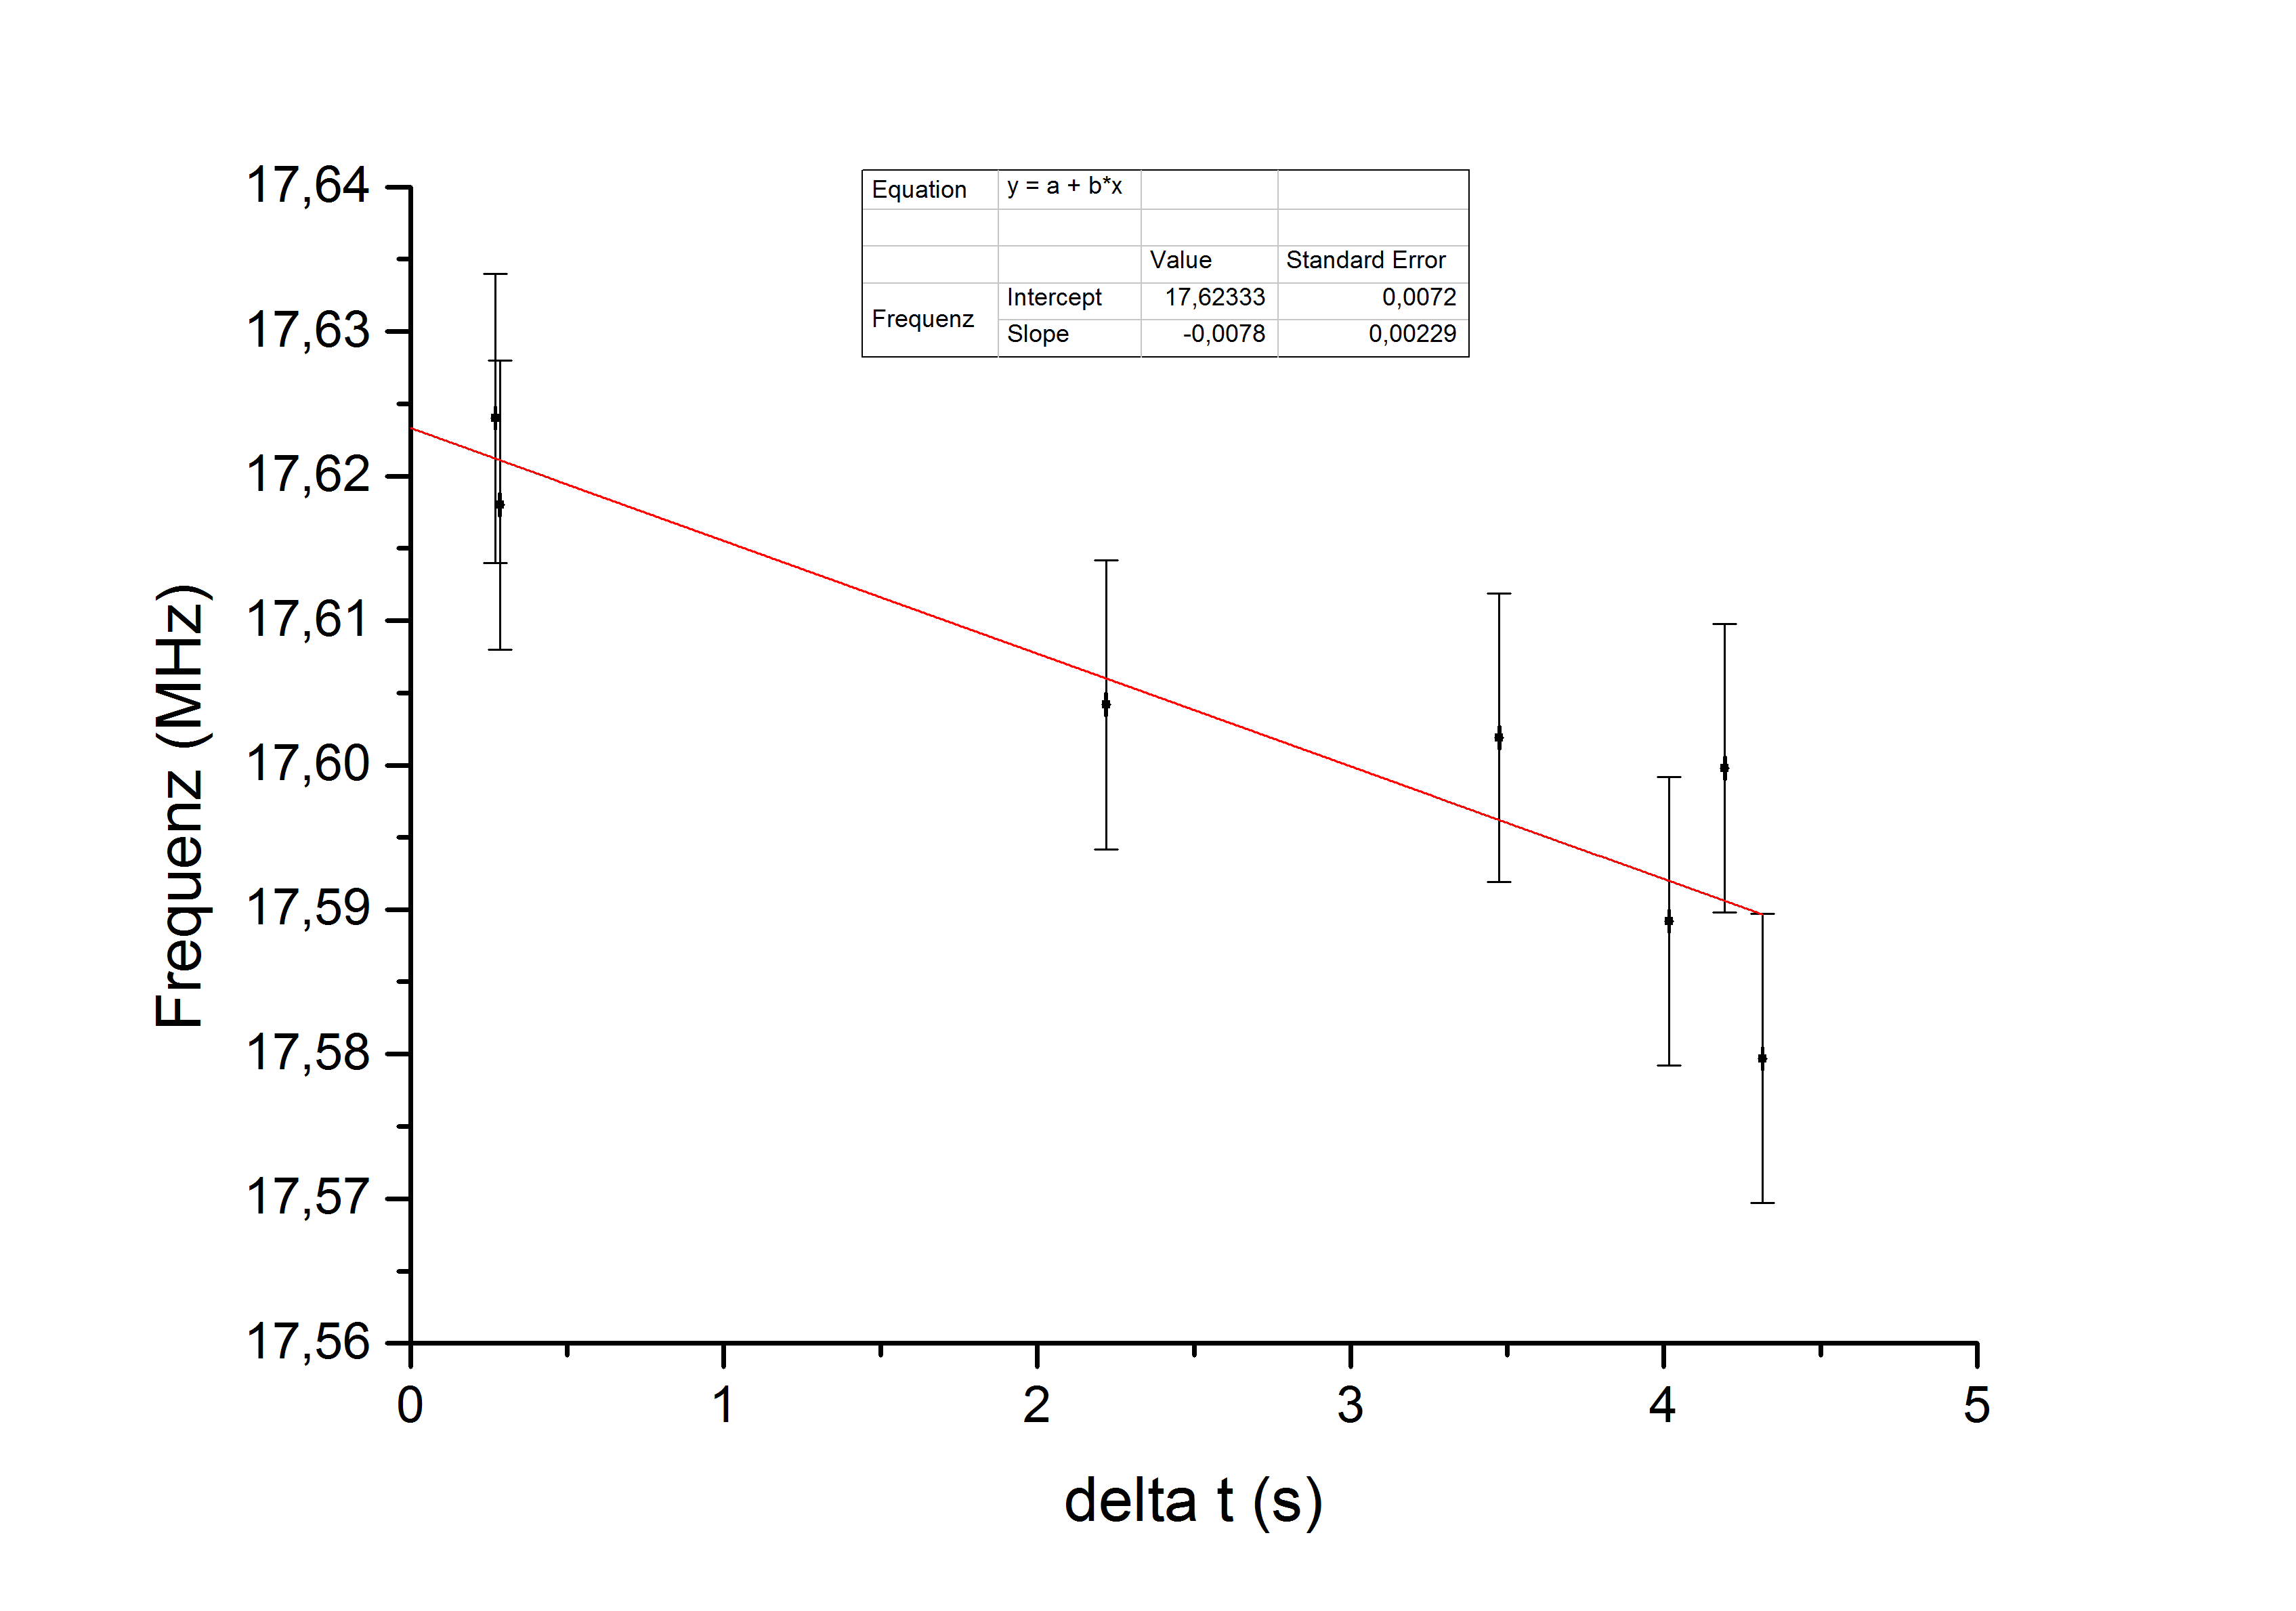
\includegraphics[scale=0.5] {Bilder/linfit}
 \caption{Linear fit used for the determination of the resonance frequency}
 \end{center}
 \end{figure}
 \clearpage
 The scattering of the measured values is quite large due to the fact that the frequency couldn't be determined very accurately. \\
The resonance frequency we determined using this method is $\nu=(17,623\pm0,007) MHz$. Using $B=(419\pm0,8)mT$, for the gyromagnetic ratio we get:\\
\[\nu=\frac{\gamma\cdot B}{2\pi}\]
\[\Leftrightarrow \gamma=\frac{\nu\cdot2\pi}{B}\]
\[\Rightarrow s_{\gamma}=\sqrt{(\frac{\partial \gamma}{\partial B})^{2}\cdot s_{B}^{2}+(\frac{\partial\gamma}{\partial\nu})^{2}\cdot s_{\nu}^{2}}=\sqrt{\frac{4\pi^{2}\cdot\nu^{2}}{B^{4}}\cdot s_{B}^{2}+\frac{4\pi^{2}}{B^{2}}\cdot s_{\nu}^{2}}\]
With this formula, using the lock-in method we get the following for the gyromagnetic ratio:\\
$\gamma=(2,643\pm0,005)\cdot 10^{8}\frac{1}{s\cdot T}$ \\
A discussion of this result can be found in the chapter "Conclusion".


%Inhaltsverzeichnis
\end{document}
